\chapter{Evaluating a time feedback notification to manage information interruptions}

\begin{mynote}
\subsubsection{Chapter outline}
This chapter describes two studies that, given varying IACs, explore the extent to which a design intervention that shows time information can influence people's strategies, speed and accuracy. Study 5 evaluates these with an experimental task, to see if making design changes influence the strategies people adopt, and can make people adopt more accurate and faster. Study 6 evaluates them in the office setting, to ascertain how appropriate the proposed recommendations are for a naturalistic task for which they would be used.

Together these studies intend to show that the new interface makes people switch less between entering and looking up information, which makes them faster to complete the data entry task overall and can reduce errors.
\end{mynote}

\section{Study 6: Looking up information in email during an online data entry task}

\subsection{Introduction}
%BRIDGE WITH LAST CHAPTER
\begin{comment}
The findings of the previous studies will have given insight into the influence of IAC on people's strategies of managing looking up information and how different strategies may be more efficient and accurate than others. For example, one finding can be that people who look up information from high IAC sources as they need it are slower and make more data entry errors than people who first collect all information and then enter it all in one sequence. 
It will have highlighted some functionalities that a data entry expenses system needs to offer users. These findings are translated into a set of requirements. These are used to test the existing system against, and used to develop possible future design recommendations suited to the task of entering expenses. 

The design recommendations will take into account both findings from Study 3 and 4 on what influences people's strategies and what is desirable, as well as the setting studied in Study 1 and 2 and what is feasible. For example, desired changes in the actual interface may be too expensive to be realistic, and it may be more feasible to change the way information sources are designed, or how these are laid out in the user's environment. Screenshots of the current interface system will be used (initial ones were obtained in Study 1, additional ones will be obtained in Study 2). 

Study 5 aims to test different designs in a controlled experiment, to investigate if changing design features influences people's switching strategies and their speed and accuracy in data entry. It will use the same task paradigm as Study 4 and compare different designs, to see if these changes have an influence on the strategies people adopt in looking up information for a data entry task, and whether these changes can make people adopt strategies that improve accuracy. 
\end{comment}

%INTRODUCTION TO CURRENT
Data entry is a common task in work settings. In many cases, people have to access multiple sources to find, collect, and enter information \citep{Borghouts2017}. When users have to switch between sources, it is often difficult to maintain focus on the task \citep{Gonzalez2004}. It opens up opportunities to get distracted, and a switch to look up information may take longer than intended. In addition, people can further self-interrupt their work for unrelated activities \citep{Jin2009}.
In order to improve focus and mitigate self-interruptions, \citet{Kim2017} developed an intervention that allowed people to temporarily block specific sources that they considered distracting, such as email, IM applications and social media. However often these sources then needed to be accessed after all for the task they were working on. Other commercial applications do not block sources but instead provide users an overview of their computer activities, to reflect how much time they spend in total on tasks, and certain sources ("ManicTime," 2018, "RescueTime," 2018). However, as these tools provide information of past usage, it is often not clear to users what they have to do with the data (Collins, Cox, Bird, & Cornish-Tresstail, 2014), and there is little evidence of their effectiveness in improving focus (Whittaker, Hollis, & Guydish, 2016). Gould, Cox and Brumby (2016) looked at switching behaviour during online crowdsourcing work, and found that an intervention during work that encouraged people to stay focused after people had interrupted reduced number of switches to unrelated tasks. Recognising that switches occur as part of the task, we consider whether the duration of switches can be reduced by giving people real-time feedback on how long they switch away for during a data entry task. This is important to consider, because the longer people interrupt, the more disruptive it is (Monk, Trafton, & Boehm-Davis, 2008), and the harder it is to resume a task (Altmann, Trafton, & Hambrick, 2017).
This study aims to investigate whether an intervention showing people how long they switch on average has an effect on the duration and number of switches during a data entry task. An online experiment was conducted where participants had to complete a data entry task. Participants had to enter numeric codes into a form, which they had to retrieve from a message sent to their personal email. We deliberately chose to present the information as a message in participants' email inboxes, as email is an integral part of data entry work but known to be a source of distraction, and people often spend more time on it than originally intended (Hanrahan & Pérez-Qu, 2015; Mark, Iqbal, Czerwinski, Johns, & Sano, 2016). We therefore expected it to have a distracting effect during the switches to look up information. Half of the participants received feedback on the average length of their switches through a browser notification. Our results show that the experimental group who received a notification made shorter switches than the control group. In addition, they completed the data entry task faster and made fewer data entry errors. 

\subsection{Method}
\subsubsection{Participants}
Thirty-two participants (19 women) took part in the online experiment. Ages ranged from 22 to 63 (M = 29.7 years, SD = 8.6 years). The participants were recruited via university email lists, social media and online platforms to advertise academic studies. 

\subsubsection{Design}
The study used a between-participants design with one independent variable, a notification. In the control condition, participants did not receive a notification, but switches away from the data entry window were recorded. In the notification condition, participants were shown a notification every time they completed a trial. This notification showed how long on average they were away for when switching away from the window, before returning to the task. The purpose of this notification was to see if the number and duration of switches could be reduced by giving participants feedback on the time spent of on switches. Dependent variables were number and duration of switches away from the data entry interface, trial completion time, and data entry errors. Switching behaviour was recorded using JavaScript's blur and focus events. These were triggered whenever a participant switched away from the data entry window, whether to their email inbox or to a different window or application. 

\subsubsection{Materials}
The task used was based on a common routine data entry task involving processing expenses (Borghouts et al., 2017). Participants were presented with an online sheet containing a set of ten 'expenses' (see Figure 1). They had to complete each row by entering the correct expense code for the expense. They retrieved this code by looking it up in a table of 25 expense categories which each had a corresponding 5-digit expense code, shown in Figure 2. Participants had to determine which category an expense belonged to, look up the code of this category and enter it in the row of the expense. We used expense categories and codes that are currently used by a public university to process expenses.

In the example of Figure 1, the expense in the top row belongs to the category 'Postage' and the participant would have to copy the code 22104 from the expense table into the empty cell of the top row. A code did not occur more than once in a trial. The codes within a trial could be entered in any order. 
Once the codes of the ten expenses had been entered, participants clicked the Next button to go to the next trial and the sheet was filled with ten new expenses. Participants were not alerted to any mistakes and once they had pressed 'Next', they could not return to the previous trial to correct any errors. Participants had to complete one practice trial, and five experimental trials. The purpose of the practice trial was for the participant to get familiar with the task, and the recorded data from this trial was excluded from the analysis.

The experiment was conducted in a web browser. In addition to the main task, we implemented a browser notification that appeared when participants in the notification condition switched away from the data entry window (see Figure 3). Every time participants switched, a notification appeared at the right-hand corner of their screen that told participants how long on average they go away for when they switch. The notification stayed visible for several seconds as set by default by the browser, or participants could dismiss the notification themselves by clicking on it.

\subsubsection{Procedure}
The study was advertised online with a brief description and a website link to sign up. Participants signed up for the experiment by entering their email address, and were sent an email with the table of expense categories and expense codes. The email also included instructions with a new link where the study was available. Participants were asked to complete the task on a desktop or laptop computer and open the experiment in Google Chrome, Firefox or Safari. Participants were not informed beforehand which condition they had been allocated to, and were told the purpose of the study was to understand how people perform data entry tasks. Participants in the notification condition were informed that they would receive notifications during the experiment. 
Participants first read an online consent form on the website, and were not able to continue to the experiment until they had agreed to the consent form. Participants in the notification condition received an additional dialog box to enable notifications in their browser, and had to click 'OK' to continue. Participants were instructed to have both their email and data entry window open on the same device, and to keep both windows maximised at all time, to ensure they had to switch back and forth between the two windows. Participants who made no recorded switches would be excluded from the dataset. 
After completing all experimental trials, participants were shown a page of debriefing information, explaining the purpose of the study. An email address was included as a point of contact if participants had any further questions. Participants took between 10 and 20 minutes to complete the experiment.

\subsection{Results}
Table \ref{tbl:ch56-Table1} summarises the results of the conditions in terms of the four dependent variables. The number of switches, length of switches and the error rate were not normally distributed, so non-parametric Mann-Whitney tests were used to analyse effects of a notification on these dependent variables. A Shapiro-Wilk test suggested that the trial completion times were normally distributed, W = 0.94, p = 0.05, so an independent t-test was used to analyse the effect on trial times. 
Figure \ref{fig:ch56-Figure2} shows the variability of duration of switches for the two conditions. Results show that switches were significantly shorter among participants who had a notification (M=4.51s, SD=1.80s) than among those without a notification (M=7.11s, SD=3.14s), U(17, 15) = 186, p = 0.01. There was no significant difference in number of switches, U(17, 15) = 80, p = 0.1.
Error rates were calculated by dividing the number of data entry errors divided by error opportunities. The error rates were significantly lower for participants with a notification (M=2\%, SD=2\%) compared to participants who had no notification (M=6\%, SD=6\%), U(17, 15) = 190, p < .01. Participants with a notification were also faster in completing trials (M=94.98s, SD=17.69s) compared to participants without a notification (M=122.90s, SD=35.43s), t(30) = 2.96, p < .01.

\begin{table}
\caption{Means and standard deviations of dependent variables for each condition.}
\centering
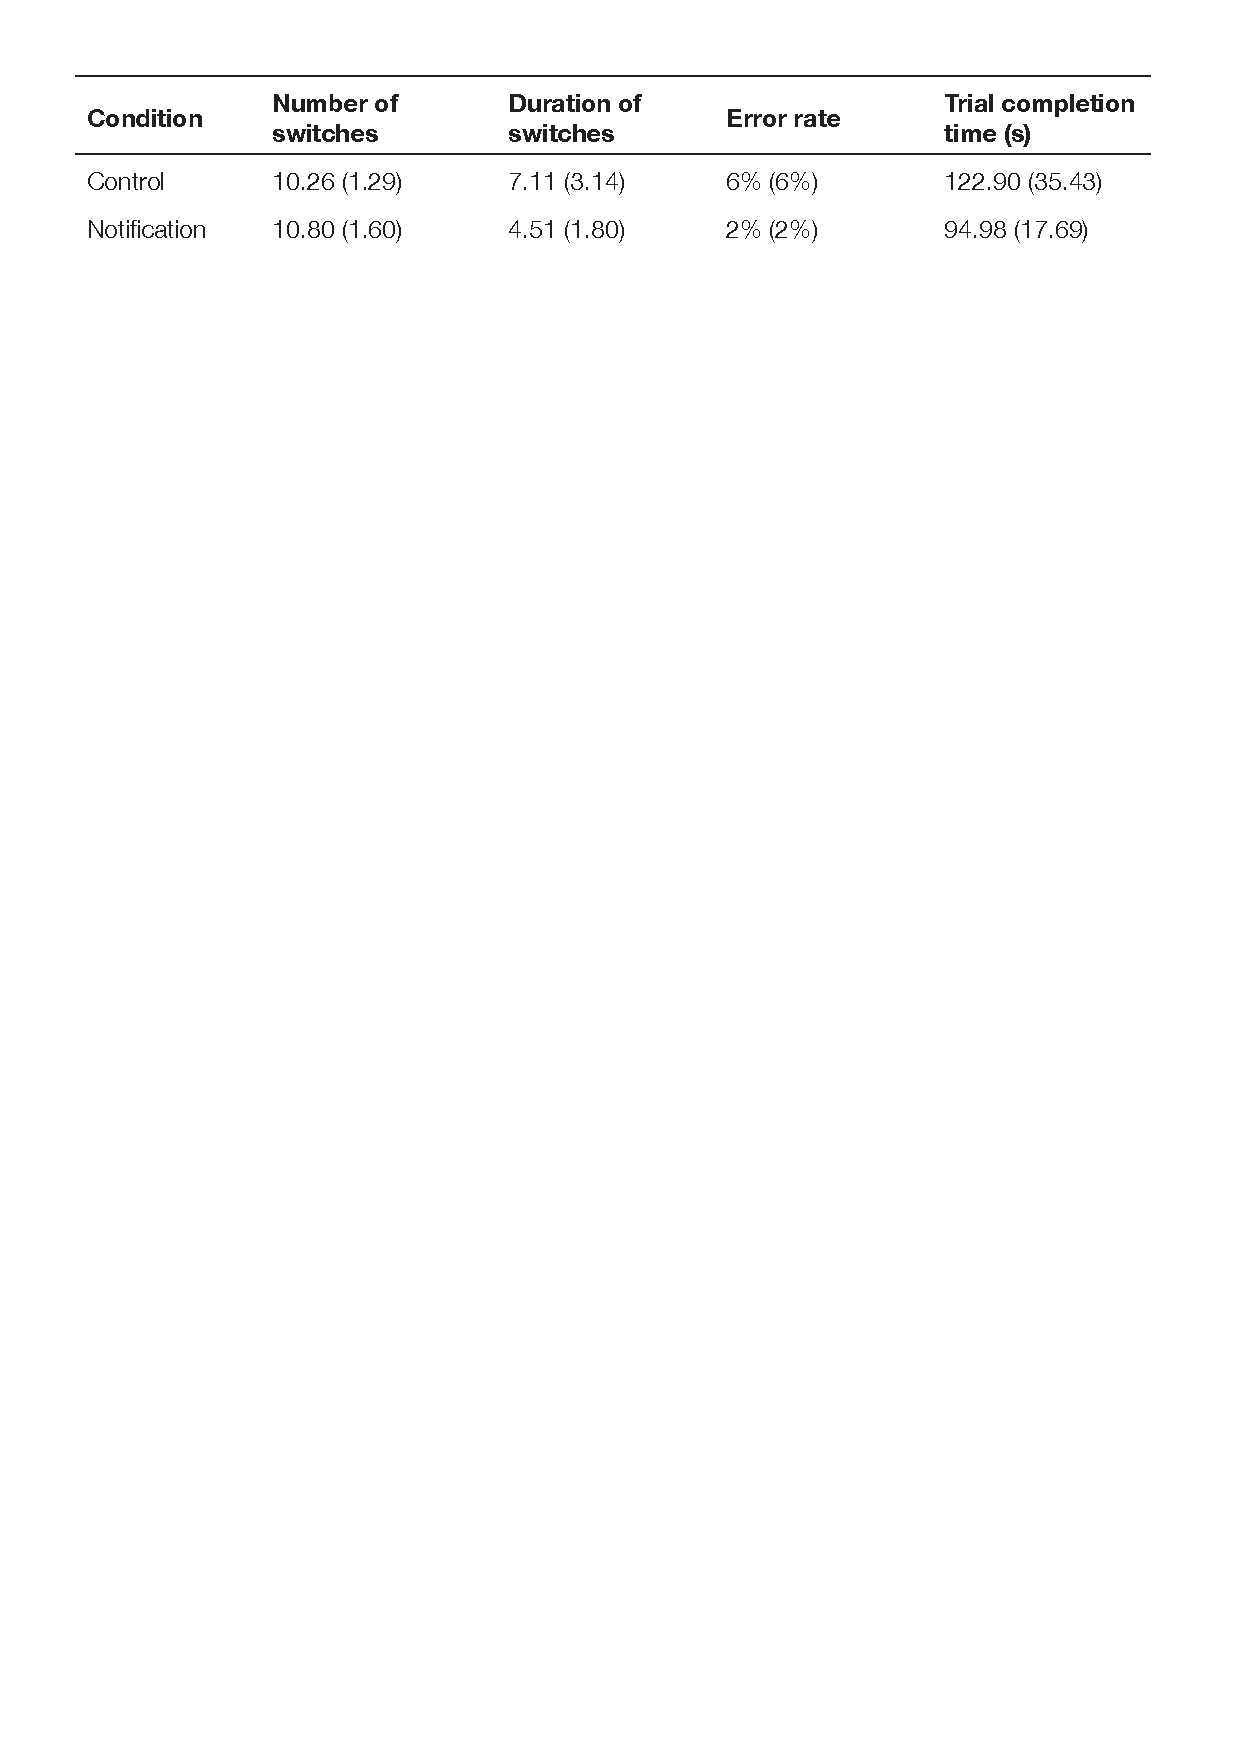
\includegraphics[width=0.9\textwidth]{images/ch56/ch56-Table1.pdf}
\vspace{-3pt}
\label{tbl:ch56-Table1}
\end{table}

\begin{figure}
\centering
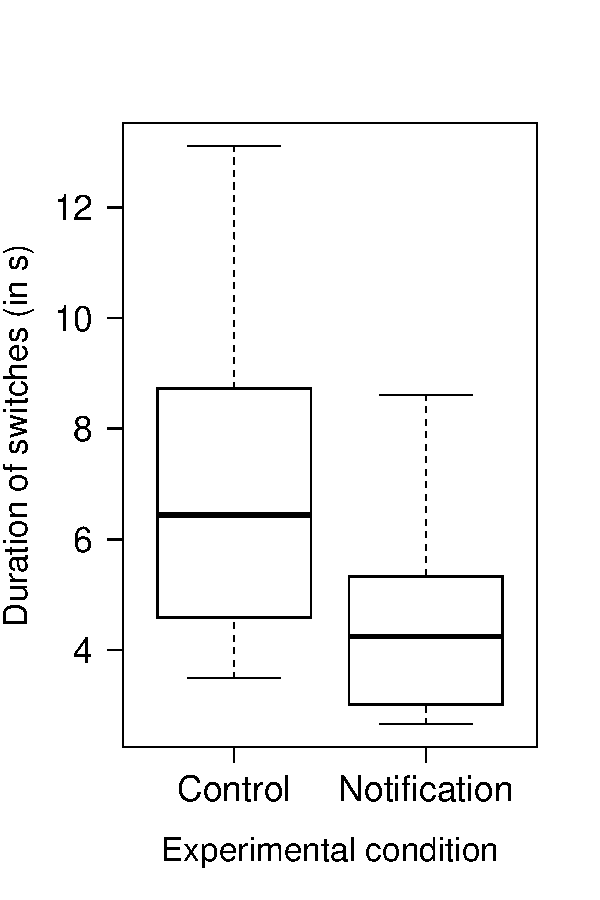
\includegraphics[width=0.2\textwidth]{images/ch56/ch56-Figure2.pdf}
\caption{Boxplot of duration of switches away from the data entry interface in each condition.}
%\vspace{-3pt}
\label{fig:ch56-Figure2}
\end{figure}

\subsection{Discussion}
The aim of this study was to see whether showing people how long they switch on average reduces the number and length of their switches. The results show that people can benefit from receiving feedback on the length of their switches: participants made shorter switches, were faster to complete the task, and made fewer errors. These findings suggest that shorter switches can lead to better task performance, and are in line with previous studies connecting the duration of an interruption to its disruptiveness \citep{Altmann2017, Monk2008}.

Nevertheless, as even short interruptions can have a negative effect on performance (Altmann, Trafton, & Hambrick, 2014), it was also measured if the number of switches were reduced. Interestingly, feedback on switching duration did not reduce the number of switches as in prior work (Gould et al., 2016). This could be explained by the moment in the task that people received feedback. In Gould et al.'s study, feedback appeared after every switch. Participants may have tried to reduce switches, either because they were more aware of every switch or because they wanted to avoid the message. In contrast to our study, their participants were not supposed to switch, so the number of switches was lower. In the current study participants were switching more often as they had to as part of the task: on average, they switched once for every data entry (i.e., ten times per trial). Giving notifications at every switch would have had the risk of overexposing participants to notifications and limiting its usefulness (Cutrell, Czerwinski, & Horvitz, 2001; Whittaker et al., 2016). Therefore, feedback was only given after every trial. Future data entry studies that require fewer switches are needed to see if a notification upon every switch can reduce both the number and length of switches. Moreover, because the notification only showed information regarding the duration of switches, participants may have focused on reducing the duration, rather than number of switches. 

The current study used focus and blur events to analyse switching behaviour. This meant that task switches outside the device, with the task window still in focus, were not captured. Possibly participants learnt to not interrupt themselves when they were away from this window, but after they had returned to the window. Without an accurate estimate of how long participants should take to complete the task, it is difficult to determine moments at which participants were away from their computer (Rzeszotarski, Chi, Paritosh, & Dai, 2013).  Using other techniques, such as prompts at random intervals to confirm people are still working on the task, may be able to give a further insight whether our intervention changes overall self-interruption behaviour. 

Most studies on self-interruptions introduced an artificial distraction, such as chat messages, to measure when, how long, and how often people self-interrupt to attend to this distracting task (Katidioti & Taatgen, 2013; Salvucci & Bogunovich, 2010). The current study makes a small methodological contribution by using participants' own personal email inbox, based on the assumption that email provides a source of distraction (Hanrahan & Pérez-Qu, 2015; Mark et al., 2016). However, in our study, participants only needed to find and open an email once. Once they had this email opened, they did not have to re-find it in their inbox for the remainder of the experiment, and may have had this email maximised on their screen, hiding incoming messages. In practice however, people have to first find the email in their inbox, which can partly contribute to the distraction. Our study has already shown an effect on behaviour by switching to an email inbox. We expect there to be a higher potential for distraction if people have to also find the correct email in their inbox.

The results of our experiment indicate that showing people how long they switch on average reduces the duration of switches and can improve people's task performance. The work makes a contribution to our understanding of switching behaviour for routine data entry tasks to distracting, but task-relevant, applications such as email. Our results also suggest ways in which tendencies to attend to distractions might be mitigated, and can provide a useful pointer for the design of productivity interventions to improve focus. In the current study, an experimental task was used in order to measure task performance. We plan on running a follow-up study with participants doing their own data entry work, to evaluate whether the positive effect of time feedback on people's switching behaviour can extend to naturalistic tasks. 



\section{Study 7: Looking up information for expenses}

\subsection{Introduction}
%BRIDGE FROM LAST STUDY
Study 6 aims to evaluate the design recommendations in a finance office with workers, to see how appropriate and feasible the proposed recommendations would be in the context for which they are developed. Depending on what the design recommendations will be, I will take them through a prototype, which can be a paper prototype, storyboard, or digital mockup, and if possible I will ask them to perform the task with and without the proposed changes. 

In order to understand whether the notification will work in a less controlled setting, the study will be replicated with data entry workers doing expenses work. They will be asked to install the plug-in in their browser and use it when they are processing expenses. Participants can use the add-in to select the browser page which shows the expenses system as the 'main task page'. Every time they switch away from this page, or if the page is inactive for more than x seconds, a JavaScript event will be triggered to log the timestamp. This event will be triggered again when the user returns to the page. The timestamps will be used (and stored in an online spreadsheet?) to determine the number and duration of interruptions.
To observe the effect of time feedback, the participants will be divided into a control and experimental group. 
The experimental group will be asked to install the plug-in and will receive a notification. If the main task page is not in focus, either because participants have switched to another page or if it has been inactive for x seconds, they will receive a notification with a warning message. Upon returning to the expenses page, they will receive a notification indicating how long they were away from the page. The control group will be asked to install the plug-in, but will receive no notifications. It is explained that the purpose of the study is to log people's switching behaviour, and participants will be able to see their data at the end of the study.
Participants will be asked to use the add-in for one week in which they have to do a substantial amount of expenses work, and keep a diary of their experiences. Within a week of finishing the diary, a follow-up interview will be scheduled to gather more detailed explanations of participants' experiences of using the add-in.

The study aims to address the following research question: does feedback on interruption length have an effect on people's self-interruption behaviour for expenses work in a finance office setting? 

\subsection{Method}
\subsubsection{Participants}
Ten participants took part in the study. They were recruited via the same recruitment methods as Study 1 and 2: they were invited via email.
Participants were reimbursed with a \pound20 Amazon voucher.

\subsubsection{Materials}
ManicTime was used to measure people's switching behaviour. This is an application that allows users to reflect on their application and web usage. 

\subsubsection{Procedure}
Participants were asked to install ManicTime on their work computer for two weeks. They were told the purpose of the study was to see how people switch between applications, documents and computer windows for expenses tasks. In the first week, they were told that they were free to choose if, when and how often to look at the information, but that it was important to complete at least one expenses task.

In the second week, participants in the experimental condition were asked to install the browser extension. They were instructed that they had to complete at least one expenses task, using the extension. Participants in the control condition were asked to complete at least one expenses task in the first week, and one expenses task in the second week, in order to compare if any measured changes were due to the browser extension or participants becoming more aware of their switching behaviour after reflecting on their information. 

After two weeks, participants were interviewed about their experience of using the tools. In particular, they were asked whether the information was useful and whether it changed anything in how they went about their work. During the interview, they were asked to share their database and discuss it. The database was saved for further analysis. It was instructed that if the database contained any sensitive data, they would be assisted in removing any or all of the application names. Participants were also still eligible to participate, if they did not wish to share their database.

The interviews took about 40 minutes and were audio recorded.

\subsubsection{Data analysis}
The ManicTime database of each participant was used to analyse people's switching behaviour. 

\subsection{Findings}

\subsection{Discussion}

\subsection{Contributions}
\begin{itemize}
\item
Development of design recommendations for an expenses system.
\item
Demonstrate how an understanding of the used information sources and people's switching strategies between entering and looking up information can be used to adapt the design of the data entry interface. 
\item
Demonstrate the applicability of design recommendations in the financial office settings in which the expenses task is currently done. 
\item
Demonstrate that design features can influence people's strategies in entering expenses in a financial office setting.
\end{itemize}

